\documentclass[11pt,a4paper,oneside]{report}


\usepackage{amsmath,amssymb,calc,ifthen}

\usepackage{float}

\usepackage[table,usenames,dvipsnames]{xcolor} % for coloured cells in tables

\usepackage{tikz}

% Allows us to click on links and references!

\usepackage{hyperref}
\hypersetup{
    colorlinks,
    citecolor=black,
    filecolor=black,
    linkcolor=black,
    urlcolor=black
}

% Nice package for plotting graphs
% See excellent guide:
% http://www.tug.org/TUGboat/tb31-1/tb97wright-pgfplots.pdf
\usetikzlibrary{plotmarks}
\usepackage{amsmath,graphicx}
\usepackage{epstopdf}
\usepackage{caption}
\usepackage{subcaption}

% highlight - useful for TODOs and similar
\usepackage{color}
\newcommand{\hilight}[1]{\colorbox{yellow}{#1}}

\newcommand\ci{\perp\!\!\!\perp} % perpendicular sign
\newcommand*\rfrac[2]{{}^{#1}\!/_{#2}} % diagonal fraction

\usepackage{listings}



% margin size
\usepackage[margin=1in]{geometry}

\tikzstyle{state}=[circle,thick,draw=black, align=center, minimum size=2.1cm,
inner sep=0]
\tikzstyle{vertex}=[circle,thick,draw=black]
\tikzstyle{terminal}=[rectangle,thick,draw=black]
\tikzstyle{edge} = [draw,thick]
\tikzstyle{lo} = [edge,dotted]
\tikzstyle{hi} = [edge]
\tikzstyle{trans} = [edge,->]


\definecolor{mygreen}{rgb}{0,0.6,0}
\definecolor{mygray}{rgb}{0.5,0.5,0.5}
\definecolor{mymauve}{rgb}{0.58,0,0.82}

\lstset{ %
  backgroundcolor=\color{white},   % choose the background color; you must add 
%\usepackage{color} or \usepackage{xcolor}
  basicstyle=\footnotesize,        % the size of the fonts that are used for the 
%code
  breakatwhitespace=false,         % sets if automatic breaks should only happen 
%at whitespace
  breaklines=true,                 % sets automatic line breaking
  captionpos=b,                    % sets the caption-position to bottom
  commentstyle=\color{mygreen},    % comment style
  deletekeywords={...},            % if you want to delete keywords from the 
%given language
  escapeinside={\%*}{*)},          % if you want to add LaTeX within your code
  extendedchars=true,              % lets you use non-ASCII characters; for 
%8-bits encodings only, does not work with UTF-8
  frame=single,                    % adds a frame around the code
  keepspaces=true,                 % keeps spaces in text, useful for keeping 
%indentation of code (possibly needs columns=flexible)
  keywordstyle=\color{blue},       % keyword style
  language=Octave,                 % the language of the code
  morekeywords={*,...},            % if you want to add more keywords to the set
  numbers=left,                    % where to put the line-numbers; possible 
%values are (none, left, right)
  numbersep=5pt,                   % how far the line-numbers are from the code
  numberstyle=\tiny\color{mygray}, % the style that is used for the line-numbers
  rulecolor=\color{black},         % if not set, the frame-color may be changed 
%on line-breaks within not-black text (e.g. comments (green here))
  showspaces=false,                % show spaces everywhere adding particular 
%underscores; it overrides 'showstringspaces'
  showstringspaces=false,          % underline spaces within strings only
  showtabs=false,                  % show tabs within strings adding particular 
%underscores
  stepnumber=2,                    % the step between two line-numbers. If it's 
%1, each line will be numbered
  stringstyle=\color{mymauve},     % string literal style
  tabsize=2,                       % sets default tabsize to 2 spaces
  title=\lstname                   % show the filename of files included with 
%\lstinputlisting; also try caption instead of title
}


\title{Graphical Models Coursework 1}
\author{
    Razvan Valentin Marinescu\\
    \texttt{razvan.marinescu.14@ucl.ac.uk}
    \and
    David Owen\\
    \texttt{david.owen.14@ucl.ac.uk}
    \and
    Kin Quan\\
    \texttt{kin.quan.10@ucl.ac.uk}
}

\begin{document}
\belowdisplayskip=12pt plus 3pt minus 9pt
\belowdisplayshortskip=7pt plus 3pt minus 4pt

\maketitle{}


\section*{Problem 2.5}
Define the set of nodes as $\left\{x_{1}, \ldots , x_{n} \right\}$ where $n$ is the number of nodes in DAG and the edges of DAG is defined as $\left\{ (x_{i},x_{j}) | x_{i} \rightarrow x_{j}, i \neq j \right\}$. \\
\newline
Let us find the ancestors of a node $x_{i}$.
\begin{enumerate}
	\item Look at each of the edge in the DAG, if the edge is of the form $(x_{k},x_{i})$ then go to the next step, if not then stop.
	\item Repeat the same process for every $x_{k}$ until you come to a stop.
	\item List the nodes.
\end{enumerate}
This gives a list of ancestors for $x_{i}$ in the DAG.

\section*{Problem 2.6}

The histogram is generated using the Floyd-Warshall algorithm. This finds the minimum distance between all pairs of nodes on a directed graph. In order to apply this to the Wikipedia data, the adjacency matrix is first made symmetrical (i.e. undirected), to reflect that $i$ knowing $j$ implies $j$ knows $i$, as stated in the question.


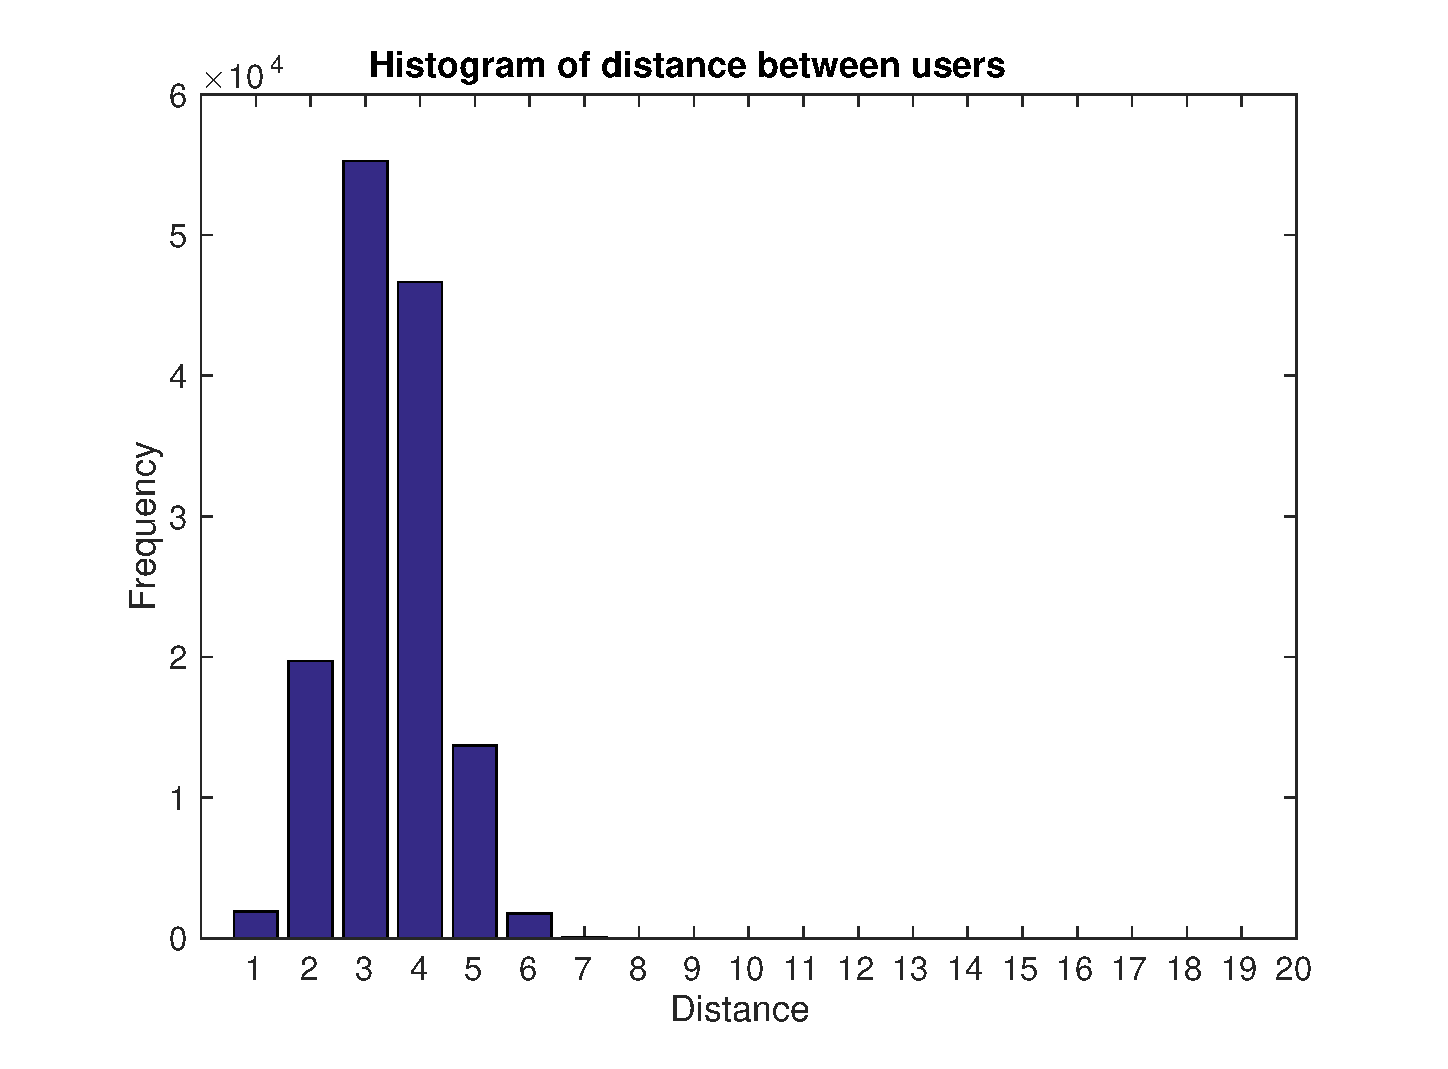
\includegraphics[scale=0.6]{plots/206_histogram}


\begin{lstlisting}
using MAT
using PyPlot

vars = matread("/Users/davido/code/BRML/data/WikiAdjSmall.mat")

# get adjacency matrix
V = vars["A"]

# make a new copy of V, which will be processed to be symmetric and [0,1]
V_new = copy(V)

# make adjacency matrix symmetric, because we assume it's undirected
for i in 1:size(V_new)[1]
        for j in 1:size(V_new)[2]
                if (V[i,j]==1) || (V[j,i]==1)
                        V_new[i,j] = 1
                        V_new[j,i] = 1
                elseif ((V[i,j]!=0) && (V[j,i]!=0))
                        println(i,",",j)
                        error("CANNOT TRANSFORM TO ADJACENCY MATRIX!")
                end
        end
end

# initialise distances matrix at Inf for every pair
dists = ones(size(V_new)) * Inf

# Floyd-Warshall loop: figure out the minimum distance from each node to every other node
for i in 1:size(dists)[1]
        dists[i,i] = 0
end

for i in 1:size(dists)[1]
        for j in 1:size(dists)[1]
                if V_new[i,j] > 0
                        dists[i,j] = V_new[i,j]
                end
        end
end

for i in 1:size(dists)[1]
        for j in 1:size(dists)[1]
                for k in 1:size(dists)[1]
                        if dists[j,k] > dists[j,i] + dists[i,k]
                                dists[j,k] = dists[j,i] + dists[i,k]
                        end
                end
        end
end

# extract relevant output -- can't just hist() whole matrix, because diagonals are irrelevant
output = Float64[]

for i in 1:size(V_new)[1]
        for j in 1:size(V_new)[2]
                if i < j
                        push!(output, dists[i,j])
                end
        end
end

h = PyPlot.plt.hist(output, 0:1:20)

\end{lstlisting}

\section*{Problem 2.7}


\section*{Problem 2.9}
Let $N=3n$ where $n$ is an integer, let us prove the hypothesis by induction on $n$. Consider $n=1$ i.e. when $N=3$. This is trivial as there is three nodes with no edges therefore there are three cliques that are form. Let us now assume that the hypothesis is true for for $N$ therefore there exist a graph $G$ such that it displays all the properties stated in the question. To prove the hypothesis let us consider the graph $G$ and introduce a new partition of three nodes. For each node in the partition let us connect it to every node in $G$. Therefore the maximal cliques will contain $N-1$ edges furthermore there will only exist $3^{N/3}$ maximal cliques otherwise to form a new maximal cliques a node in $G$ would have to connect another node in the same partition. Thus for each of the three newly introduced node there would be $3^{N/3}$ maximal cliques thus the total maximal cliques is $3(3^{N/3}) = 3^{(N+1)/3}$. Thus the hypothesis is proved.

\section*{Problem 3.3}

\begin{itemize}
 \item $tuberculosis \ci smoking\;|\; shortness\;of\;breath$ is \textbf{false}, 
because path $t \to e \to d \to b \to s$ is not blocked
 \item $lung\;cancer \ci  bronchitis\;|\;smoking$ is \textbf{true}, because:
  \begin{itemize}
    \item path $l \to s \to b$ is blocked ($s$ is instantiated)
    \item path $l \to e \to d \to b$ is blocked (has collider ${e,d,b}$)
  \end{itemize}
 \item $visit \; to \; Asia \ci smoking\;|\;lung\;cancer$ is \textbf{true}, 
because:
   \begin{itemize}
    \item path $a \to t \to e \to l \to s$ is blocked ($l$ is instantiated)
    \item path $a \to t \to e \to d \to b \to s$ is blocked ($d$ is 
uninstantiated)
  \end{itemize}
 \item $visit \; to \; Asia \ci smoking\;|\;lung \; cancer; \; shortness \; of 
\; breath$ is \textbf{false} because path $a \to t \to e \to d \to b \to s$ is 
not blocked ($d$ is instantiated).
\end{itemize}



\section*{Problem 3.4}


\section*{Problem 3.8}
\begin{enumerate}
	\item 
	\begin{enumerate}
		\item Let us find $p(B=tr|W=tr)$, by Bayes' rule:
		\begin{align}
		p(B=tr|W=tr) &= \frac{p(B = tr , W = tr)}{p(W =tr)} \\
		&= \frac{p(W = tr | B = tr)p(B = tr)}{p(W=tr)} \\
		&= \frac{p(W = tr | B = tr)p(B = tr)}{\sum_{A, B}~p(W = tr| A)p(A|B)}\\		
		\end{align}
	To find $p(W = tr | B = tr)$ lets us use Bayes' rule again:
	\begin{align}
	p(W = tr | B = tr) &= \sum_{A} p(A|B=tr)p(W = tr|A)\\
	&= 0.99\times0.9+(1-0.99)\times0.5\\
	&= 0.896.
	\end{align}
	Combining the results from above gives:
	\begin{align}
	p(B=tr|W=tr) &= \frac{0.896\times0.01}{0.01\times(0.99\times0.9+0.01\times 0.5)+0.99(0.05\times 0.9 + 0.95\times 0.5)}\\
	&= 0.0171.
	\end{align}
	\item
	Lets find $p(B=tr|W=tr,G=fa)$, by Bayes' rule:
	\begin{equation}
	p(B=tr|W=tr,G=fa) = \frac{p(W=tr, G=fa | A)\times p(B=tr)}{p(W=tr, G=fa)}
	\end{equation}
	Let us find $p(W=tr, G=fa | A)$,
	\begin{align}
	p(W=tr, G=fa | A) &= \sum_{A} p(W=tr, G=fa |A)p(A|B=tr)\\
	&=0.9 \times 0.3 \times 0.99+ 0.5\times 0.8 \times 0.01\\
	&= 0.2713
	\end{align}
	Combining the results from above gives:
	\begin{align}
	p(B=tr|W=tr,G=fa) &= \frac{0.2713 \times 0.01}{\sum_{A,B}~p(W=tr |A) p(G=fa|A) p(A|B)}\\
	&= {0.002713}\times(0.01\times (0.99 \times 0.9 \times 0.3 + 0.01 \times 0.5 \times 0.8) \nonumber \\
	&+0.99\times(0.05 \times 0.9 \times 0.3 + 0.95 \times 0.9 \times 0.8))^{-1}\\
	&= 0.004.
	\end{align}
	\end{enumerate}
	\item Since $\tilde{G} = fa$ then $p(G=fa) = 0.9$ and  $p(G=tr) = 0.1$. Also since $\tilde{W} = tr$ then $p(W=fa) = 0.7$ and $p(W=tr)=0.3$.
	\begin{enumerate}
		\item Let us find $p(B=tr | \tilde{W})$.
		\begin{equation}
		p(B=tr | \tilde{W}) = \sum_{W} p(B= tr|W)p(W |\tilde{W})
		\end{equation}
		In order to compute the above, let us first compute $p(B=tr|W=fa)$. By Bayes' law:
		\begin{align}
		p(B=tr|W=fa) &= \frac{p(W=fa|B=tr)p(B=tr)}{p(W=fa)}\\
		&= \frac{(1-0.896)\times 0.01}{1-0.523}\\
		&= 0.002.
		\end{align}
		Thus from above
		\begin{align}
		p(B=tr | \tilde{W}) &= 0.3\times 0.017 + 0.7 \times 0.002\\
		&=0.007
		\end{align}
		\item
		Let us find $p(B=tr|\tilde{W},\tilde{G})$, since $W$ and $G$ are independent then
		\begin{equation}
		p(B=tr|\tilde{W},\tilde{G}) = \sum_{W,G} {p(B=tr|W,G) p(W|\tilde{W}) p(G|\tilde{G})}.
		\end{equation}
		By Bayes' rule;
		\begin{equation}
		p(B=tr|\tilde{W},\tilde{G}) = \sum_{W,G} \frac{p(W,G|B=tr) p(B=tr) p(W|\tilde{W}) p(G|\tilde{G})}{p(W,G)}.
		\end{equation}
		In order to compute the above, we require to compute the following:
		\begin{enumerate}
			\item
			\begin{align}
			p(W=tr, G=tr|B=tr) &= p(W=tr|B=tr)p(G=tr|B=tr),\\
			&= \sum_{A} p(W=tr, A|B=tr) p(G=tr, A|B=tr),\\
			&= 0.99 \times 0.9 \times 0.7 + 0.01 \times 0.5 \times 0.2,\\
			&= 0.625.
			\end{align}
			\item
			\begin{align}
			p(W=fa, G=tr|B=tr) &= p(W=fa|B=tr)p(G=tr|B=tr),\\
			&= \sum_{A} p(W=fa, A|B=tr) p(G=tr, A|B=tr),\\
			&= 0.99 \times 0.1 \times 0.7 + 0.01 \times 0.5 \times 0.2\\
			&= 0.070.
			\end{align}
			\item
			\begin{align}
			p(W=fa,G=fa|B=tr)&= p(W=fa|B=tr) p(G=fa|B=tr)\\
			&= \sum_{A} p(W=fa, A|B=tr) p(G=fa, A|B=tr),\\
			&= 0.99\times 0.1 \times 0.3 + 0.01 \times 0.5 \times 0.8,\\
			&= 0.034.
			\end{align}
			\item
			\begin{align}
			p(W=tr,G=fa|B=tr)&= p(W=tr|B=tr) p(G=fa|B=tr)\\
			&= \sum_{A} p(W=tr, A|B=tr) p(G=fa, A|B=tr),\\
			&= 0.99 \times 0.9 \times 0.3 + 0.01 \times 0.5 \times 0.8,\\
			&= 0.271
			\end{align}
			\item
			\begin{align}
			p(W=tr,G=tr)&=\sum_{B} p(W=tr,G=tr|B)p(B) \\
			&=0.131
			\end{align}
			\item
			\begin{align}
			p(W=tr,G=fa)&=\sum_{B} p(W=tr,G=fa|B)p(B) \\
			&= 0.380
			\end{align}
			\item
			\begin{align}
			p(W=fa,G=tr)&= \sum_{B} p(W=tr,G=fa|B)p(B)\\
			&=0.098.
			\end{align}
			\item
			\begin{align}
			p(W=fa,G=fa)&= \sum_{B} p(W=fa, G=fa|B)p(B) \\
			&=0.378.
			\end{align}
		\end{enumerate}
		Hence using all the above gives:
		\begin{align}
		p(B=tr|\tilde{W},\tilde{G}) = 0.031
		\end{align}
	\end{enumerate}
\end{enumerate}

\section*{Problem 3.9}

\subsection*{1. Belief network}

\begin{figure}[H]
  \centering
    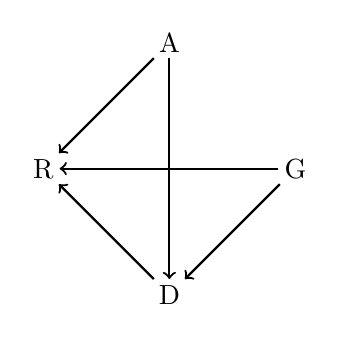
\begin{tikzpicture}[scale=0.8,help lines/.style={color=lightgray,line 
width=0.2pt},post/.style={->,shorten >=1pt,>=stealth',thick}]
    
    \node[inner sep=2] (A) at (0.0,2.0){A};
    \node[inner sep=2] (G) at (2.0,0.0) {G};
    \node[inner sep=2] (R) at (-2.0,0.0) {R};
    \node[inner sep=2] (D) at (0.0,-2.0) {D};

    \draw[->, thick] (A) -- (R);
    \draw[->, thick] (A) -- (D);
    \draw[->, thick] (G) -- (D);
    \draw[->, thick] (G) -- (R);
    \draw[->, thick] (D) -- (R);
    
    \end{tikzpicture}
    \caption{Belief network}
    \label{fig:all_trade_cca_black}     
\end{figure}

\subsection*{2. Computation of $p(R=tr \; | \; D=tr)$}

By considering the generative model and marginalising we get 
\begin{equation}
p(R=tr \; | \; D=tr) = \sum\limits_{A,G} p(R=tr \;
| A, \; G,\; D=tr) p(A) p(G) p(D=tr \; | \; G, \; A)
\end{equation}

This suggests that from a database of patient entries we 
take the number of patients who received the drug \emph{and} recovered, and
then divide it by the total number of patients who received the drug. 

\subsection*{3. Computation of $p(recover \; | \; do(drug),\; young)$}

The do-calculus allows us to deal with interventional studies, in which we
have specifically \emph{set} a causal condition in the experiment. The causal
variable (here $D$) is set to its interventional value, and then severed from
its parent variables. This yields the following new DAG:


\begin{figure}[H]
  \centering
    \begin{tikzpicture}[scale=0.8,help lines/.style={color=lightgray,line 
width=0.2pt},post/.style={->,shorten >=1pt,>=stealth',thick}]
    
    \node[inner sep=2] (A) at (0.0,2.0){A};
    \node[inner sep=2] (G) at (2.0,0.0) {G};
    \node[inner sep=2] (R) at (-2.0,0.0) {R};
    \node[inner sep=2] (D) at (0.0,-2.0) {D};

    \draw[->, thick] (A) -- (R);
    \draw[->, thick] (G) -- (R);
    \draw[->, thick] (D) -- (R);
    
    \end{tikzpicture}
    \caption{Belief network}
    \label{fig:do_calc_DAG}    
\end{figure}

Hence, from the generative model
\begin{equation}
p(R=tr \; | \; do(drug),\; A=yo) =
\sum\limits_{G} p(R=tr \; | \; do(drug), \; A=yo, \; G) p(G)
\end{equation}

To calculate this, we must take the target group (young people) and then examine their
recovery results by gender. We then produce a weighted sum of their recovery
probability, weighted by the proportions of each gender in the study. 

%\hilight{David, could you please write the answer for this one?}

\section*{Problem 3.11}


\section*{Problem 3.12}
Two belief networks are Markov equivalent if they represent the same conditional
independence statements. Markov equivalence between two graphs can be determined
by calculating the graphs' \emph{skeletons} and \emph{immoralities}. If they
have the same skeleton and immoralities, the two graphs are Markov equivalent.

\begin{lstlisting}
function MarkovEquiv(A, B)
    # test skeleton
    skel_A = get_skeleton(A)
    skel_B = get_skeleton(B)

    # test immoralities
    imm_A = get_immoralities(A)
    imm_B = get_immoralities(B)

    if (skel_A==skel_B) && (imm_A==imm_B)
        return true
    else
        return false
    end
end

function get_skeleton(M)
    skel = zeros(size(M))

    for i in 1:size(M)[1]
        for j in 1:size(M)[2]
            if M[i,j] == 1
                # skeleton is undirected version of the DAG
                skel[i,j] = 1
                skel[j,i] = 1
            end
        end
    end

    return skel
end

function get_immoralities(M)
    imms = Array[]
    for i in 1:size(M)[1]
        for j in 1:size(M)[2]
            for k in 1:size(M)[1]
                # if two nodes share a child but are not directly connected, they form an immorality
                if  M[i,j] == 1 && M[k,j] == 1 &&
                    M[i,k] != 1 && M[k,i] != 1 && 
                    i != j && i != k && j != k
                        push!(imms, [i, j, k])
                end
            end
        end
    end

    # sort immoralities so identical immoralities can be removed, leaving only unique immoralities
    unique_imms = unique(map(x -> sort(x), imms))

    return unique_imms
end
\end{lstlisting}


\section*{Problem 3.13}
The skeletons are equivalently:

\begin{equation}
\begin{pmatrix}
 0.0 & 0.0 & 1.0 & 1.0 & 0.0 & 1.0 & 0.0 & 0.0 & 0.0 \\
 0.0 & 0.0 & 1.0 & 0.0 & 1.0 & 0.0 & 0.0 & 0.0 & 0.0 \\
 1.0 & 1.0 & 0.0 & 0.0 & 1.0 & 0.0 & 1.0 & 0.0 & 0.0 \\
 1.0 & 0.0 & 0.0 & 0.0 & 0.0 & 1.0 & 0.0 & 1.0 & 1.0 \\
 0.0 & 1.0 & 1.0 & 0.0 & 0.0 & 0.0 & 1.0 & 0.0 & 0.0 \\
 1.0 & 0.0 & 0.0 & 1.0 & 0.0 & 0.0 & 0.0 & 1.0 & 0.0 \\
 0.0 & 0.0 & 1.0 & 0.0 & 1.0 & 0.0 & 0.0 & 0.0 & 1.0 \\
 0.0 & 0.0 & 0.0 & 1.0 & 0.0 & 1.0 & 0.0 & 0.0 & 0.0 \\
 0.0 & 0.0 & 0.0 & 1.0 & 0.0 & 0.0 & 1.0 & 0.0 & 0.0 \\
\end{pmatrix}
\end{equation}

The immoralities are equivalently $\left( 1, 2, 3\right)$, $\left( 1, 3, 5 \right)$ and
$\left( 4, 7, 9 \right)$.

Hence the two graphs are Markov equivalent.

\section*{Problem 3.14}


\section*{Problem 3.15}

\subsection*{1.}
\begin{figure}[H]
  \centering
    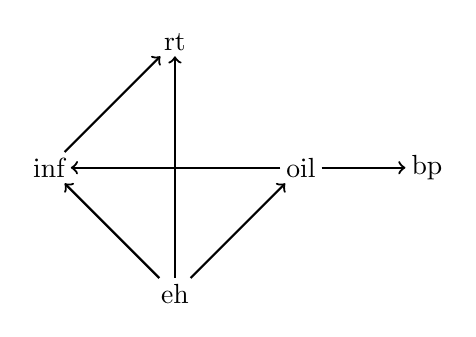
\begin{tikzpicture}[scale=0.8,help lines/.style={color=lightgray,line 
width=0.2pt},post/.style={->,shorten >=1pt,>=stealth',thick}]
    
    \node[inner sep=2] (eh) at (0.0,-2.0){eh};
    \node[inner sep=2] (oil) at (2.0,0.0) {oil};
    \node[inner sep=2] (bp) at (4.0,0.0) {bp};
    \node[inner sep=2] (inf) at (-2.0,0.0) {inf};
		\node[inner sep=2] (rt) at (0.0,2.0) {rt};

    \draw[->, thick] (oil) -- (bp);
    \draw[->, thick] (eh) -- (oil);
    \draw[->, thick] (eh) -- (inf);
    \draw[->, thick] (oil) -- (inf);
    \draw[->, thick] (eh) -- (rt);
		\draw[->, thick] (inf) -- (rt);
    
    \end{tikzpicture}
    \caption{Belief network}
    \label{fig:all_trade_cca_black}     
\end{figure}


\subsection*{2.}

The answer can be easily calculated using Julia. We first define the 
conditional probability tables and then we compute the joint distribution 
$p(eh, oil, inf, bp, rt)$. From this we calculate the marginals $p(inf,rt,bp) 
= \sum_{oil, eh}p(eh, oil, inf, bp, rt)$ and $p(rt,bp) = 
\sum_{inf}p(inf, rt, bp)$. Using these marginals we use Bayes' rule to compute 
the posterior $p(inf|rt, bp) = p(inf, rt, bp)/p(rt, bp)$. The Julia code that 
was used to compute this is given below. The final answer $p(inf = high | rt 
= high, bp = normal) = 0.984746 $\\

\begin{lstlisting}
low, high, normal = 1,2,3
E,O,I,R,B = 1,2,3,4,5

pE = PotArray(E, [2//10 8//10])
pOgE = PotArray([O E], [9//10 5//100; 1//10 95//100])


tabIgOE=zeros(2,2,2)
tabIgOE[low, low, low]=9//10
tabIgOE[low, low, high]=1//10
tabIgOE[low, high, low]=1//10
tabIgOE[low, high, high]=1//100

tabIgOE[high, low, low]=1//10
tabIgOE[high, low, high]=9//10
tabIgOE[high, high, low]=9//10
tabIgOE[high, high, high]=99//100

pIgOE = PotArray([I O E], tabIgOE)


tabRgIE=zeros(2,2,2)
tabRgIE[:, low, low]=[9//10; 1//10]
tabRgIE[:, low, high]=[1//10; 9//10]
tabRgIE[:, high, low]=[1//10; 9//10]
tabRgIE[:, high, high]=[1//100; 99//100]

pRgIE = PotArray([R I E], tabRgIE)


pBgO = PotArray([B O], [9//10 1//10; 1//10 4//10; 0//10 5//10])

pAll = pBgO * pRgIE * pIgOE * pOgE * pE

pIRB = sum(pAll, [O E])

pRB = sum(pIBR, I)

pIgRB = pIBR / pRB

\end{lstlisting}


\section*{Problem 3.17}

\subsection*{1.}

In order to prove $a \ci c$ we need to show that $p(a,c) = p(a)p(c)$. We first 
calculate the joint probability distribution $p(a,b,c) = p(c|b)p(b|a)p(a)$. 
Then 
we marginalise over $b$ to get $p(a,c)=\sum_{b} p(a,b,c) = \sum_{b} 
p(c|b)p(b|a)p(a)$. 

We will now calculate the three terms from the sum $\sum_{b} 
p(c|b)p(b|a)p(a)$. For $b=1$ we get 

% b = 1

\begin{equation}
\label{317A}
p(b = 1|a) =  
  \begin{pmatrix}
   \ 1/4 \\[0.4em]
   \ 15/40 \\
 \end{pmatrix}
\end{equation}

 
\begin{equation}
\label{317B}
    p(b = 1, a) = p(b = 1|a) p(a) = \begin{pmatrix}
      \ 3/20 \\[0.4em]
      \ 3/20 \\
    \end{pmatrix}
\end{equation}

\begin{equation}
\label{317C}
p(c | b = 1) =  
  \begin{pmatrix}
   \ 1/3 \\[0.4em]
   \ 2/3 \\
 \end{pmatrix} 
\end{equation}

Combining equations \eqref{317B} and \eqref{317C} we get:

\begin{equation}
\label{317D}
p(a, b = 1, c) =  p(c | b = 1 )p(b = 1,a)
  \begin{pmatrix}
   \ \frac{3}{20} \frac{1}{3} & \frac{3}{20} \frac{2}{3} \\[0.4em]
   \ \frac{3}{20} \frac{1}{3} & \frac{3}{20} \frac{2}{3} \\
 \end{pmatrix} = \frac{1}{40}
  \begin{pmatrix}
   \ 2 & 4 \\[0.4em]
   \ 2 & 4 \\
 \end{pmatrix} 
\end{equation}

A similar computaiton is done for $p(a, b = 2, c)$ and $p(a, b = 3, c)$. 

% b =2

\begin{equation}
\label{317E}
    p(b = 2, a) = p(b = 2|a) p(a) = 
    \begin{pmatrix}
      \ \frac{1}{12} \frac{3}{5} \\[0.4em]
      \ \frac{1}{8} \frac{2}{5} \\
    \end{pmatrix} = 
    \begin{pmatrix}
      \ 1/20 \\[0.4em]
      \ 1/20 \\
    \end{pmatrix}
\end{equation}

\begin{equation}
\label{317F}
p(c | b = 2) =  
  \begin{pmatrix}
   \ 1/2 \\[0.4em]
   \ 1/2 \\
 \end{pmatrix} 
\end{equation}

Combining equations \eqref{317E} and \eqref{317F} we get:

\begin{equation}
\label{317G}
p(a, b = 2, c) =  
  \begin{pmatrix}
   \ \frac{1}{20} \frac{1}{2} & \frac{1}{20} \frac{1}{2} \\[0.4em]
   \ \frac{1}{20} \frac{1}{2} & \frac{1}{20} \frac{1}{2} \\
 \end{pmatrix} = \frac{1}{40}
  \begin{pmatrix}
   \ 1 & 1 \\[0.4em]
   \ 1 & 1 \\
 \end{pmatrix} 
\end{equation}

%% b = 3

Now for $b = 3$ we get:

\begin{equation}
\label{317H}
    p(b = 3, a) = p(b = 3|a) p(a) = 
    \begin{pmatrix}
      \ \frac{2}{3} \frac{3}{5} \\[0.4em]
      \ \frac{1}{2} \frac{2}{5} \\
    \end{pmatrix} = \frac{1}{5}
    \begin{pmatrix}
      \ 2 \\[0.4em]
      \ 1 \\
    \end{pmatrix}
\end{equation}

\begin{equation}
\label{317I}
p(c | b = 3) =  
  \begin{pmatrix}
   \ 15/40 \\[0.4em]
   \ 5/8 \\
 \end{pmatrix} 
\end{equation}

Combining equations \eqref{317H} and \eqref{317I} we get:

\begin{equation}
\label{317J}
p(a, b = 3, c) =  
  \begin{pmatrix}
   \ \frac{2}{5} \frac{15}{40} & \frac{2}{5} \frac{5}{8} \\[0.4em]
   \ \frac{1}{5} \frac{15}{40} & \frac{1}{5} \frac{5}{8} \\
 \end{pmatrix} = \frac{1}{40}
  \begin{pmatrix}
   \ 6 & 10 \\[0.4em]
   \ 3 & 5 \\
 \end{pmatrix} 
\end{equation}

Summing up all the right-hand side terms from equations \eqref{317D},  
\eqref{317G} and  \eqref{317J} we get

\begin{equation}
\label{317K}
p(a, c) =  \sum_{b} p(a,b,c) = \frac{1}{40}
  \begin{pmatrix}
   \ 9 & 15 \\[0.4em]
   \ 6 & 10 \\
 \end{pmatrix} 
\end{equation}
 
From the joint distribution $p(a,c)$ we can calculate the marginalise

\begin{equation}
\label{317L}
p(c) =  \sum_{a} p(a,c) = \frac{1}{8}
  \begin{pmatrix}
   \ 3 \\[0.4em]
   \ 5 \\
 \end{pmatrix} 
\end{equation}
 
Using the given distribution $p(a)$ and the above equation we can now calculate:
\begin{equation}
\label{317M}
p(a)p(c) =
  \begin{pmatrix}
   \ \frac{3}{5} \frac{3}{8} & \frac{3}{5} \frac{5}{8} \\[0.4em]
   \ \frac{2}{5} \frac{3}{8} & \frac{2}{5} \frac{5}{8} \\
 \end{pmatrix} = \frac{1}{40}
  \begin{pmatrix}
   \ 9 & 15 \\[0.4em]
   \ 6 & 10 \\
 \end{pmatrix} 
\end{equation}

From equations \eqref{317K} and \eqref{317M} it results that $p(a,c) = p(a)p(c)$ 
which implies $a \ci c$

\subsection*{2.}

We are given that:

\begin{equation}
\label{317N}
p(a,b,c) = \frac{1}{Z}\phi(a, b)\psi(b,c). 
\end{equation}
Looking at the element at position $(i,j)$ in the $MN^\top$ matrix we notice 
that:
\begin{equation}
\frac{1}{Z}\left[ MN^\top \right]_{ik} = \frac{1}{Z}\sum_{j}\phi(a=i, 
b=j)\psi(b=j, c=k). 
\end{equation}
Applying equation \eqref{317N} in the right hand side term above we get:
\begin{equation}
\frac{1}{Z}\sum_{j}\phi(a=i, b=j)\psi(b=j, c=k) = \sum_{j}p(a = i, b = j, c = k) 
= p(a = i, c = k) 
\end{equation}
which implies that
\begin{equation}
\frac{1}{Z}\left[ MN^\top \right]_{ik} = p(a = i, c = k) 
\end{equation}

\subsection*{3.}

Using the given and the result from the previous subpoint we get
\begin{equation}
 \frac{1}{Z}\left[ MN^\top \right] = m_0n_0^\top = p(a, c) 
\end{equation}
and $\forall i,j$
\begin{equation}
 m_0(i)n_0(j) = p(a=i, c=j) 
\end{equation}
If we define functions $f(i)=m_0(i)$ and $g(j)=n_0(j)$, $\forall i \in dom(a), j 
\in dom(c)$ then we get:
$$ p(a,c) = \frac{1}{Z}f(a)g(c)$$ which implies $a \ci c$

\subsection*{4.}

$\forall (i,j) \in dim(MN^\top)$ we have:
$$MN^\top(i,j) = \sum_{k=1}^{3}M(i,k)N^\top(k,j) = \sum_{k=1}^{3} m_k(i)n_k(j) = 
m_1n_1^\top(i,j) + m_2n_2^\top(i,j) + m_3n_3^\top(i,j)$$  
which implies that:
$$ MN^\top = m_1n_1^\top + m_2n_2^\top + m_3n_3^\top$$

\subsection*{5.}

From the previous results and from the definitions of $m_2$ and $n_3$ we get:
$$MN^\top = m_1n_1^\top + m_2n_2^\top + m_3n_3^\top = m_1n_1^\top + \lambda 
m_1n_2^\top + m_3\gamma(n_1^\top + \lambda n_2^\top)$$
Factorising further we get
$$MN^\top = m_1(n_1^\top + \lambda n_2^\top) + m_3\gamma (n_1^\top + \lambda 
n_2^\top) = (m_1 + \gamma m_3)(n_1^\top + \lambda n_2^\top) = m_0n_0^\top$$

\subsection*{6.}

Let us set $\lambda = 1$ and $\gamma = 1$ and the following vectors:

$m_1 =   
 \begin{pmatrix}
   \ 2  \\[0.4em]
   \ 1  \\
 \end{pmatrix} 
$  
$m_2 =   
 \begin{pmatrix}
   \ 2  \\[0.4em]
   \ 1  \\
 \end{pmatrix} 
$  
$m_3 =   
 \begin{pmatrix}
   \ 0  \\[0.4em]
   \ 3  \\
 \end{pmatrix} 
$  
$n_1 =   
 \begin{pmatrix}
   \ 2  \\[0.4em]
   \ 2  \\
 \end{pmatrix} 
$  
$n_2 =   
 \begin{pmatrix}
   \ 1  \\[0.4em]
   \ 3  \\
 \end{pmatrix} 
$  
$n_3 =   
 \begin{pmatrix}
   \ 3  \\[0.4em]
   \ 5  \\
 \end{pmatrix}
 $\\\\
This gives us the following matrices:

$ M = 
 \begin{pmatrix}
   \ 2 & 1 \\[0.4em]
   \ 2 & 1 \\[0.4em]
   \ 0 & 3
 \end{pmatrix}
$
$ N^\top = 
 \begin{pmatrix}
   \ 2 & 1 & 3 \\[0.4em]
   \ 2 & 3 & 5
 \end{pmatrix}
$\\\\
Setting $p(a) = 
 \begin{pmatrix}
   \ 1/2 \\[0.4em]
   \ 1/2
 \end{pmatrix}
$ gives the following conditional tables:

$ p(b|a) = \begin{pmatrix}
   \ 1/2 & 1/5 \\[0.4em]
   \ 1/2 & 1/5 \\[0.4em]
   \ 0 & 3/5
 \end{pmatrix} 
$
$ p(c|b) = \begin{pmatrix}
   \ 1/2 & 1/4 & 3/8 \\[0.4em]
   \ 1/2 & 3/4 & 5/8
 \end{pmatrix} 
$

Running the following code in Julia (using the BRML toolbox) shows that $p(a,c) 
= p(a)p(c)$ which implies $a \ci c$. The code was adapted from 
\texttt{demoChainIndepRational.jl}

\begin{lstlisting}
A,B,C=1,2,3

pA = PotArray(A, [1//2, 1//2])

pBgA = PotArray([B A], [1//2 1//5; 1//2 1//5; 0 3//5])

pCgB = PotArray([C B], [1//2 1//4 3//8; 1//2 3//4 5//8])

pABC = pCgB * pBgA * pA
pAC = sum(pABC, B)

pA=sum(pAC,C)
pC=sum(pAC,A)

println("pAC-pA*pC=")
println(pAC-pA*pC)

\end{lstlisting}


\section*{Problem 3.20}

We use BRML toolbox to calculate:
$$p(w,h,inc) = p(w|inc)p(h|inc)p(inc)$$
$$p(w,h,inc = low) = 
\begin{pmatrix}
 14/125 & 56/125 & 0 & 0\\
  6/125 & 24/125 & 0 & 0\\
  0   &  0   & 0 & 0\\
  0   &  0   & 0 & 0
\end{pmatrix}
$$
$$p(w,h,inc = high) = 
\begin{pmatrix}
 0 & 0 & 3/250 &  7/250\\
 0 & 0 & 3/500 &  7/500\\
 0 & 0 & 3/125 &  7/125\\
 0 & 0 & 9/500 & 21/500
\end{pmatrix}
$$

We then calculate the marginal:

$$p(w,h) = \sum_{inc}p(w,h,inc) = 
\begin{pmatrix}
 14/125 & 56/125 & 3/250 &  7/250\\
  6/125 & 24/125 & 3/500 &  7/500\\
  0    & 0   & 3/125 &  7/125\\
  0    & 0   & 9/500 & 21/500
\end{pmatrix}
$$

Further marginalising over $w$ and $h$ we get:

$$p(w) = \sum_{h}p(w,h) = 
\begin{pmatrix}
  3/5\\
  13/50\\
  2/25\\
  3/50
\end{pmatrix}
$$

$$p(h) = \sum_{w}p(w,h) = 
\begin{pmatrix}
4/25\\
16/25\\
3/50\\
7/50
\end{pmatrix}
$$

$$p(w,h) - p(w)p(h) = 
\begin{pmatrix}
  2/125 &   8/125 & -3/125 &  -7/125\\
  4/625 &  16/625 & -6/625 & -14/625\\
 -8/625 & -32/625 & 12/625 &  28/625\\
 -6/625 & -24/625 &  9/625 &  21/625
\end{pmatrix} \neq 0_{4,4}
$$

which implies that  $h \not\!\perp\!\!\!\perp w$. Now we will show that $ w 
\ci h | inc$ :

$$ p(w,h| inc) = \frac{p(w,h,inc}{p(inc)} $$

$$ p(w,h | inc = low) = 
\begin{pmatrix}
 7/50 & 14/25 & 0 & 0\\
 3/50 &  6/25 & 0 & 0\\
 0   & 0  & 0 & 0\\
 0   & 0  & 0 & 0\\
\end{pmatrix}
$$

$$ p(w,h | inc = high) = 
\begin{pmatrix}
 0 & 0 & 3/50  &  7/50\\ 
 0 & 0 & 3/100 &  7/100\\
 0 & 0 & 3/25  &  7/25 \\
 0 & 0 & 9/100 & 21/100\\
\end{pmatrix}
$$

$$p(w,h|inc) - p(w|inc)p(h|inc) = 0_{4,4,2}
$$

which implies that $ w \ci h | inc$ . 
\begin{lstlisting}
w,h,inc=1,2,3
low,high=1,2,3

pInc = PotArray(inc, [8//10 2//10])
pWgI = PotArray([w inc], [7//10 2//10; 3//10 1//10; 0 4//10; 0 3//10])
pHgI = PotArray([h inc], [2//10 0; 8//10 0; 0 3//10; 0 7//10])

pWHI = pWgI * pHgI * pInc
pWH = sum(pWHI, inc)

pW = sum(pWH, h)
pH = sum(pWH, w)

println("pWH - pW*pH= should not be zero")
pWH - pW*pH

pWHgI = pWHI / pInc

println("pWHgI - pWgI*pHgI= should be zero")
pWHgI - pWgI*pHgI


\end{lstlisting}


\section*{Problem 3.21}


\section*{Problem 3.22}


\section*{Extra Problem A}


\section*{Extra Problem B}


\end{document}
